% !TeX spellcheck = en_US
\documentclass[a4paper,12pt]{article}
\usepackage[utf8x]{inputenc}
\usepackage{wrapfig}
\usepackage{graphicx}
\usepackage{float}
\usepackage{listings}
\usepackage{amsmath}
\usepackage{caption}
\usepackage{subcaption}
\usepackage[usenames,dvipsnames,svgnames,table]{xcolor}
\usepackage{datetime}
\usepackage{fancyhdr}
\pagestyle{fancy}

% Title Page
\title{AST3310 Project 2}
\author{Andreas Ellewsen}

\fancyhead[L]{Andreas Ellewsen}
%\fancyhead[C]{Modeling the solar core}
\fancyhead[R]{Spring 2015}

\begin{document}

\maketitle
\tableofcontents
\newpage
\section{Project}
The first project involved modeling the core and radiative zone of the sun. 
Obviously the sun doesn't have just these two parts.
Because of this fact, this second project involves modeling the convective zone of the sun.
The convective zone goes from the top of the radiative zone out to the surface.
This project does not consider what happens on the surface, only the interior.

\section{Assumptions}
All the assumptions from the first project still apply.
It is assumed that the radius of a parcel of gas is half of its mixing length $(r_p = l_m/2)$.
The mixing length is defined to be $l_m = \alpha H_P$, where $\alpha$ is a constant between $1/2$ and $2$, and $H_P$ is the pressure scale height.
It should also be noted that I make the assumption that all energy transport happens in the radial direction from the center of the star. 
This means that all the gradients in the angular directions are zero at every point.
\section{Calculations}
To include convection in the model I need to find equations for the energy transport through the star. This is done in a series of steps through three exercises found in the lecture notes. Before we do all of that we can find the temperature gradient needed for pure radiation by using the equation I used in the first project.
There we found that 
\begin{equation}
 \frac{\partial T}{\partial m} = -\frac{3\kappa L}{256\pi^2\sigma r^4 T^3}
\end{equation}
since we don't want the gradients with regards to mass anymore, I calculate the following:
\begin{equation*}
\begin{aligned}
 m = \frac{4\pi r^3}{3}\rho\\
 \frac{\partial m}{\partial r} = 4\rho \pi r^2 
\end{aligned}
\end{equation*}
The gradients are defined such that
\begin{equation}
 \nabla = -\frac{H_P}{T}\frac{\partial T}{\partial r}
\end{equation}
and thus we can insert all of this and find
\begin{equation*}
\begin{aligned}
 \nabla_{rad} &= -\frac{H_P}{T}\frac{\partial T}{\partial m} \frac{\partial m}{\partial r}\\
 &= \frac{H_P}{T}\frac{3\kappa L}{256\pi^2\sigma r^4 T^3}4\rho \pi r^2 
\end{aligned}
\end{equation*}
which if one does some straightforward algebra becomes
\begin{equation}
  \nabla_{rad} =\frac{3H_P\kappa L\rho}{64\pi\sigma r^2 T^4}
\end{equation}



The first one involves inserting equations \ref{F_R} and \ref{F_C} into equation \ref{F_R +F_C}, and getting an expression between $\nabla$, $\nabla_{rad}$ and $\nabla^*$. 
I also need to find an expression for the pressure scale height, and insert part of it into the equation I get from the former.
\begin{equation}
F_R = \frac{4acGT^4 m}{3\kappa Pr^2}\nabla
\label{F_R}
\end{equation}
\begin{equation}
 F_C = \rho c_P T \sqrt{g\delta}H_P^{-\frac{3}{2}}\bigg(\frac{l_m}{2}\bigg)^2(\nabla - \nabla^*)^{\frac{3}{2}}
 \label{F_C}
\end{equation}
\begin{equation}
 F_R + F_C = \frac{4acGT^4 m}{3\kappa Pr^2}\nabla_{rad}
 \label{F_R +F_C}
\end{equation}
Where $\nabla_{rad}$ is the temperature gradient needed for all the energy to be transported by radiation alone. 
$\nabla$ is the actual temperature gradient in the star.
$\nabla^*$ is the temperature gradient of a packet of gas.
$l_m$ is the mixing length.
$H_P$ is the pressure scale height.
And the rest of the symbols have their regular meanings.

To start with I need to calculate the scale height:
\begin{equation}
 H_P = -P \frac{\partial r}{\partial P}
\end{equation}

\begin{equation*}
 \frac{\partial P}{\partial r} = \frac{\partial P}{\partial m}\frac{\partial m}{\partial r} = -\frac{Gm}{4\pi r^4} 4\pi r^2 \rho = -\frac{Gm\rho}{r^2}
\end{equation*}
where I have used the expression for $\frac{\partial m}{\partial r}$, we found earlier, and
\begin{equation*}
 \frac{\partial P}{\partial m} = -\frac{Gm}{4\pi r^4}
\end{equation*}
which I have from the first project.
Inserting this into the equation for the pressure scale height gives:
\begin{equation}
 H_P = \frac{Pr^2}{Gm\rho}
\end{equation}
Now I have equations for everything one needs to find the expression between $\nabla$, $\nabla_{rad}$ and $\nabla^*$.

Thus it is time to insert \ref{F_R} and \ref{F_C} into \ref{F_R +F_C}:
\begin{equation*}
\begin{aligned}
 F_R + F_C &= \frac{4acGT^4 m}{3\kappa Pr^2}\nabla_{rad}\\
\rho c_P T \sqrt{g\delta}H_P^{-\frac{3}{2}}\bigg(\frac{l_m}{2}\bigg)^2(\nabla - \nabla^*)^{\frac{3}{2}} &= \frac{4acGT^4 m}{3\kappa Pr^2}\nabla_{rad} - \frac{4acGT^4 m}{3\kappa Pr^2}\nabla\\
\rho c_P T \sqrt{g\delta}H_P^{-\frac{3}{2}}\bigg(\frac{l_m}{2}\bigg)^2(\nabla - \nabla^*)^{\frac{3}{2}} &= \frac{4acGT^4 m}{3\kappa Pr^2}(\nabla_{rad} - \nabla)\\
(\nabla - \nabla^*)^{\frac{3}{2}} &= \bigg(\frac{2}{l_m}\bigg)^2\frac{ H_P^{\frac{3}{2}}}{\sqrt{g\delta}}\frac{4acGT^3 m}{3\rho c_P\kappa Pr^2}(\nabla_{rad} - \nabla)\\
(\nabla - \nabla^*)^{\frac{3}{2}} &= \bigg(\frac{2}{l_m}\bigg)^2 H_P\sqrt{\frac{H_P}{g\delta}}\frac{4acGT^3 m}{3\rho c_P\kappa Pr^2}(\nabla_{rad} - \nabla)\\
(\nabla - \nabla^*)^{\frac{3}{2}} &= \bigg(\frac{2}{l_m}\bigg)^2 \frac{Pr^2}{Gm\rho}\sqrt{\frac{H_P}{g\delta}}\frac{4acGT^3 m}{3\rho c_P\kappa Pr^2}(\nabla_{rad} - \nabla)\\
(\nabla - \nabla^*)^{\frac{3}{2}} &= \bigg(\frac{1}{l_m}\bigg)^2 \sqrt{\frac{H_P}{g\delta}}\frac{64\sigma T^3}{3\rho^2 c_P\kappa}(\nabla_{rad} - \nabla)\\
(\nabla - \nabla^*)^{\frac{3}{2}} &= \bigg(\frac{1}{l_m}\bigg)^2 U(\nabla_{rad} - \nabla)\\
\end{aligned}
\end{equation*}
which finally gives
\begin{equation}
 (\nabla - \nabla^*)^{\frac{1}{2}} = \bigg[\bigg(\frac{1}{l_m}\bigg)^2 U(\nabla_{rad} - \nabla)\bigg]^{1/3}
\label{xi_1}
\end{equation}
where 
\begin{equation*}
 U = \frac{64\sigma T^3}{3\kappa\rho^2 c_P}\sqrt{\frac{H_P}{g\delta}}
\end{equation*}

The next step is to insert equation (5.73) from the lecture notes into
\begin{equation}
 (\nabla^* - \nabla_{ad} ) = (\nabla -\nabla_{ad} ) - (\nabla - \nabla^* )
\end{equation}
For reference equation (5.73) is:
\begin{equation*}
 (\nabla^* - \nabla_{ad}) = \frac{32\sigma T^3}{3\kappa\rho^2 c_P v}\frac{S}{dQ}(\nabla - \nabla^*)
\end{equation*}
where $S$ is the surface area of the parcel, $d$ the diameter, and $Q$ the surface area normal to the velocity.

It is also convenient to use equation (5.78) from the lecture notes which states that:
\begin{equation*}
 v = \sqrt{\frac{g\delta l_m^2}{4H_P}}(\nabla - \nabla^*)^{1/2}
\end{equation*}

By assuming that the parcel is perfectly spherical, the geometric factor $S/dQ$ can be calculated:
\begin{equation*}
 S = 4\pi r^3\\
\end{equation*}
\begin{equation*}
 Q = \pi r^2
\end{equation*}
\begin{equation*}
 \frac{S}{dQ} = \frac{4\pi r_p^2}{2r_p\pi r_p^2} = \frac{2}{r_p}
\end{equation*}

Setting these equal, and inserting $v$, and $S/dQ$ yields:
\begin{equation*}
 \begin{aligned}
  \frac{32\sigma T^3}{3\kappa\rho^2 c_P \sqrt{\frac{g\delta l_m^2}{4H_P}}}\frac{S}{dQ}(\nabla - \nabla^*)^{1/2} = (\nabla -\nabla_{ad} ) - (\nabla - \nabla^* )\\
  \frac{64\sigma T^3}{3\kappa\rho^2 c_P}\sqrt{\frac{H_P}{g\delta}} \frac{1}{l_m}\frac{S}{dQ}(\nabla - \nabla^*)^{1/2} = (\nabla -\nabla_{ad} ) - (\nabla - \nabla^* )\\
  U \frac{1}{l_m}\frac{2}{r_p}(\nabla - \nabla^*)^{1/2} = (\nabla -\nabla_{ad} ) - (\nabla - \nabla^* )\\
  (\nabla - \nabla^* ) + \frac{2U}{l_m r_p}(\nabla - \nabla^*)^{1/2} - (\nabla -\nabla_{ad} ) = 0 \\
   \end{aligned}
\end{equation*}
This can be written as a second order equation with respect to $(\nabla - \nabla^*)^{1/2}$:
\begin{equation*}
 \xi^2 + b\xi + c = 0 
\end{equation*}
where $\xi = (\nabla - \nabla^*)^{1/2}$ and $b= \frac{2U}{l_m r_p}$. This has solutions
\begin{equation*}
 \xi = -\frac{U}{l_m r_p} \pm \sqrt{\bigg(\frac{U}{l_m r_p}\bigg)^2 + (\nabla - \nabla_{ad})}
\end{equation*}
The question now is which of the solutions to proceed with. Studying the right hand side reveals that in the first term all variables are positive, so the term will always be negative. The left hand side is the square root of a difference, and if $\nabla^*$ is larger than $\nabla$ the result would be complex. Because of this I assume that $\nabla$ is larger or equal to $\nabla^*$ at all times. This means that the right hand side must be $0$ or positive at all times, and this is only achieved by choosing a plus sign in front of the root. So finally we have:
\begin{equation}
 \xi = -\frac{U}{l_m r_p} + \sqrt{\bigg(\frac{U}{l_m r_p}\bigg)^2 + (\nabla - \nabla_{ad})}
 \label{xi_2}
\end{equation}
Now I have two equations for $\xi$, and I want to eliminate $\nabla$ from my equations. 
This is done by first solving equations \ref{xi_1} and \ref{xi_2} in terms of $\nabla$:
\begin{equation*}
\begin{aligned}
 \xi + \frac{U}{l_m r_p} &= \sqrt{\bigg(\frac{U}{l_m r_p}\bigg)^2 + (\nabla - \nabla_{ad})}\\
 \bigg(\xi + \frac{U}{l_m r_p}\bigg)^2 &= \bigg(\frac{U}{l_m r_p}\bigg)^2 + (\nabla - \nabla_{ad})
\end{aligned}
\end{equation*}
\begin{equation}
 \nabla = \bigg(\xi + \frac{U}{l_m r_p}\bigg)^2 - \bigg(\frac{U}{l_m r_p}\bigg)^2 +  \nabla_{ad}
\end{equation}

and
\begin{equation*}
\begin{aligned}
 \xi &= \bigg[\bigg(\frac{1}{l_m}\bigg)^2 U(\nabla_{rad} - \nabla)\bigg]^{1/3}\\
\xi^3 &= \bigg(\frac{1}{l_m}\bigg)^2 U(\nabla_{rad} - \nabla)\\
\frac{l_m^2}{U} \xi^3 &= (\nabla_{rad} - \nabla)
\end{aligned}
\end{equation*}
\begin{equation}
 \nabla = \nabla_{rad} - \frac{l_m^2}{U} \xi^3
 \label{nabla}
\end{equation}

Setting these two expressions for $\nabla$ equal gives:

\begin{equation*}
\begin{aligned}
  \nabla_{rad} - \frac{l_m^2}{U} \xi^3 &=  \bigg(\xi + \frac{U}{l_m r_p}\bigg)^2 - \bigg(\frac{U}{l_m r_p}\bigg)^2 +  \nabla_{ad}\\
  \nabla_{rad} - \frac{l_m^2}{U} \xi^3 &=  \xi^2 + \frac{2U}{l_m r_p}\xi + \bigg(\frac{U}{l_m r_p}\bigg)^2 - \bigg(\frac{U}{l_m r_p}\bigg)^2 +  \nabla_{ad}\\
  \nabla_{rad} - \frac{l_m^2}{U} \xi^3 &=  \xi^2 + \frac{2U}{l_m r_p}\xi +  \nabla_{ad}\\
 -\nabla_{rad} + \frac{l_m^2}{U} \xi^3 &=  -\xi^2 - \frac{2U}{l_m r_p}\xi -  \nabla_{ad}\\
  0 &= \frac{l_m^2}{U} \xi^3 +\xi^2 +\frac{2U}{l_m r_p}\xi + (\nabla_{ad}- \nabla_{rad}) \\ 
\end{aligned}
\end{equation*}
This has given us a third degree equation for $\xi$:
\begin{equation}
 a\xi^3 + b\xi^2 + c\xi + d = 0
\end{equation}
where if one assumes that $r_p = l_m/2$, we get the following:

\begin{equation}
\begin{aligned}
 a &= \frac{l_m^2}{U}\\
 b &= 1 \\
 c &= \frac{2U}{l_m r_p} = \frac{4U}{l_m^2}\\
 d &= (\nabla_{ad}- \nabla_{rad})
\end{aligned}
\end{equation}
In general, third degree equations have three solutions. Luckily for us, two of those are complex, and the difference between two temperature gradients must be a real number. 
This leaves one solution. This solution can be written:
\begin{equation}
 \xi  = -\frac{1}{3a}\bigg(b + C + \frac{\Delta_0}{C}\bigg)
\end{equation}
where 
\begin{equation}
 C = \sqrt[3]{\frac{\Delta_1 + \sqrt{\Delta_1^2 - 4\Delta_0^3}}{2}}
\end{equation}
with 
\begin{equation*}
\begin{aligned}
\Delta_0 &= b^2 - 3ac\\
\Delta_1 &= 2b^3 - 9abc + 27a^2 d\\
\end{aligned}
\end{equation*}
and
\begin{equation*}
\begin{aligned}
 \Delta_1^2 - 4\Delta_0^3 &= -27a^2\Delta\\
\Delta &= 18abcd -4b^3 d + b^2 c^2 - 4ac^3 -27a^2 d^2
\end{aligned}
\end{equation*}

This can of course be written out, and we'll have an enormous equation to look at, but it's strictly not that important what the equation looks like. The important point is that we can calculate all of the variables in this expression and since that is the case, we have an answer to $\xi$!

It should be noted that when actually computing $\xi$ in the program this equation isn't used. Instead I use the root function in the numpy package for python 2.7. This function returns all three roots, and so I just pick out the real part of the one with imaginary part equal to zero, which is exactly the same as what one gets when calculating with the equation for $\xi$ above.

Since $\xi$ can be calculated, the answer can be inserted back into equation \ref{nabla}.
This gives us $\nabla$, since $\nabla_{rad}$ also can be calculated.

At this point I have expressions for $\nabla$, $\nabla_{rad}$, and $(\nabla - \nabla^*)^{1/2}$.

Next I need an expression for $\nabla_{ad}$. Equation (5.40) in the lecture notes states that
\begin{equation}
 \nabla_{ad} = \frac{P\delta}{T\rho c_P}
\end{equation}

To find this I need an equation of state. 
I choose to use the same one as in project 1, since everything so far points towards it being a good enough approximation.
\begin{equation}
 \rho = \frac{P\mu m_u}{kT}
\end{equation}
The logarithm of this will be needed soon so I also calculate that:
\begin{equation}
 ln(\rho) = ln(P) + ln(\mu) + ln(m_u) -ln(k) - ln(T)
\end{equation}
Next there are two variables that I will also need:
\begin{equation}
\alpha = \bigg(\frac{\partial ln(\rho)}{\partial ln(P)}\bigg)_T = 1
\end{equation}
\begin{equation}
 \delta = \bigg(\frac{\partial ln(\rho)}{\partial ln(T)}\bigg)_P = -1
\end{equation}
The last thing I need is an expression for $c_P$.
From equation (5.34) in the lecture notes we have:
\begin{equation*}
 c_P - c_V = \frac{P\delta^2}{\rho T\alpha}
\end{equation*}
It turns out that the adiabatic index for a fully ionized ideal gas is
\begin{equation}
 \gamma = \frac{c_P}{c_V} = \frac{5}{3}
\end{equation}
If we multiply with this on both sides of the equation above we get
\begin{equation*}
\begin{aligned}
 \gamma(c_P - c_V) &= \frac{\gamma P\delta^2}{\rho T\alpha}\\
 c_P(\gamma - 1) &= \frac{\gamma P\delta^2}{\rho T\alpha}\\
c_P &= \frac{\gamma P\delta^2}{\rho T\alpha}\frac{1}{(\gamma - 1)}\\
c_P &= \frac{5P}{3\rho T}\frac{3}{2}
\end{aligned}
\end{equation*}
\begin{equation}
 c_P = \frac{5P}{2\rho T}
\end{equation}
Inserting this back into the equation for $\nabla_{ad}$ gives
\begin{equation}
 \nabla_{ad} = \frac{P\delta}{T\rho}\frac{1}{c_P} = \frac{P\delta}{T\rho}\frac{2\rho T}{5P} = \frac{2}{5}
\end{equation}
At this point I have expressions for $\nabla$, $\nabla_{rad}$,  $(\nabla - \nabla^*)^{1/2}$, and $\nabla_{ad}$.
This means that if I insert the answer to $\nabla$ into the equation for $(\nabla - \nabla^*)^{1/2}$ we have equations for all four gradients:
\begin{equation}
\begin{aligned}
 (\nabla - \nabla^*)^{1/2} = \xi\\
\nabla^* = \nabla- \xi^2 
\end{aligned}
\end{equation}
To summarize, the equations I have found are:
\begin{equation}
\nabla = \nabla_{rad} - \frac{l_m^2}{U} \xi^3
\end{equation}
\begin{equation}
\nabla_{ad} = 2/5
\end{equation}
\begin{equation}
\nabla_{rad} = \frac{3H_P\kappa L\rho}{64\pi\sigma r^2 T^4}
\end{equation}
\begin{equation}
\nabla^* = \nabla- \xi^2 
\end{equation}
To finish we need to know when to use the different gradients for energy transport.
This becomes clear when one thinks about what the different gradients are.
$\nabla$ is the temperature gradient of the star when we have convection.
$\nabla_{rad}$ is the gradient when we have only radiation.
$\nabla^*$ is the gradient of the parcel of gas that moves when we have convection.
$\nabla_{ad}$ is the gradient one would have if the transport was adiabatic.
Now it is clear that there are actually only two gradients to choose from when transporting the energy.
Either it is controlled by $\nabla_{rad}$, or by $\nabla$.

The instability criterion that governs this is given by
\begin{equation}
 \nabla > \nabla_{ad}
 \label{nabla-nabla_ad}
\end{equation}
but since these two gradients usually end up very close to each other, I choose to use
\begin{equation}
 \nabla_{rad} > \nabla_{ad}
 \label{nabla_rad-nabla_ad}
\end{equation}

In conclusion this means that if the gradient for radiation only, is larger than the one for adiabatic energy transport, convection must be used.
If this is not the case, we can use the one for radiation only.
Note also that if equation \ref{nabla_rad-nabla_ad} holds, but \ref{nabla-nabla_ad} doesn't, all that will happen is that we waste some computation time.

\section{Corrections from project 1}
Since project 1 did not work as intended, a number of things were fixed before implementing the above calculations into the program.

In the first project i included changes in the number of hydrogen and helium atoms. This meant that I did a time evolution of the star which was not intended, and complicated things more than it helped.
This has been removed.
I also did a mistake when implementing the limits on the reaction rates in the program. This has been fixed so that it reflects what I wrote in the report of project 1.
Furthermore I included an approximation of the number of particles contributed by atoms larger than beryllium, to the total number of particles, which was not intended. This has been removed, and the expression for $\mu$ has been corrected for this.
The last thing that needed fixing was that I used the total derivative of the density $\rho$. This is not needed since $\rho$ can be calculated from the equation of state, and thus the total derivative is never needed.

\section{Implementing convection in the model}
The first thing to note is that all the temperature changes in the first project were with regards to mass. In this project, they are with regards to radius.
This means that instead of using a variable step in mass $dm$ as in the first project, I instead use a variable step in radius $dr$.
This is the reason why there is a difference between the equations governing change in temperature during radiation between the two projects.
This also changes the rest of the equations from project 1. When switching between the two approaches, you basically multiply all the equations by $\partial m/\partial r$.
This means that instead of having these equations from project 1:
\begin{equation*}
\begin{aligned}
\frac{\partial r}{\partial m} &= \frac{1}{4\pi r^2\rho}\\
\frac{\partial P}{\partial m} &= -\frac{Gm}{4\pi r^4}\\
\frac{\partial L}{\partial m} &= \epsilon\\
\frac{\partial T}{\partial m} &= -\frac{3\kappa L }{256\pi^2\sigma r^4 T^3}\\
\end{aligned}
\end{equation*}
we get these:
\begin{equation*}
\begin{aligned}
\frac{\partial m}{\partial r} &= 4\pi r^2\rho\\
\frac{\partial P}{\partial r} &= -\frac{Gm\rho}{r^2}\\
\frac{\partial L}{\partial r} &= 4\pi r^2\rho\epsilon\\
\frac{\partial T}{\partial r} &= -\frac{3\kappa L\rho }{64\pi\sigma r^2 T^3}\\
\end{aligned}
\end{equation*}

Since we want to look at how much of the energy is produced by the two processes, I also had to add a few lines of code to the energy function from project 1. This is implemented such that the PPI chain gets 69 \% of the energy from the first process both chains go through, while PPII gets the remaining 31\%. The rest is simply given to the one it belongs to. The 69\% comes from the fact that PPI happens 69\% of the time.

Since we want plots for the fractions of energy transport and energy production, these calculations have to be inserted into the program.

The equations used to find $F_R$ and $F_C$ are as follows:
\begin{equation}
F_R = -\frac{16}{3}\frac{\sigma T^3}{\kappa \rho}\frac{\partial T}{\partial r}
\end{equation}
\begin{equation}
F_C = \frac{L}{4\pi r^2}-F_R
\end{equation}
where $F_R$ is equation 5.12 from the lecture notes, and $F_C$ is equation 5.63 from the lecture notes rewritten.

The fractions of energy production are calculated as one would calculate any fraction of a total, such that
\begin{equation}
PP_{Ifrac} = PP_I/(PP_I + PP_{II})
\end{equation}
\begin{equation}
PP_{IIfrac} = PP_{II}/(PP_I + PP_{II})
\end{equation}
\section{Results}
\subsection{Energy production}
If the energy production behaves as expected we should see almost zero output, until we reach the core. And when we get there it should increase exponentially. During all of this it is the first part of the chains that generate the most energy, and so one would expect the line for PPI in the graph to fill about 69\% of the total production all the way through. If we look at the plot generated by the program we get the plot in figure \ref{fig:Energy pruduction} which confirms this. 
\begin{figure}[H]
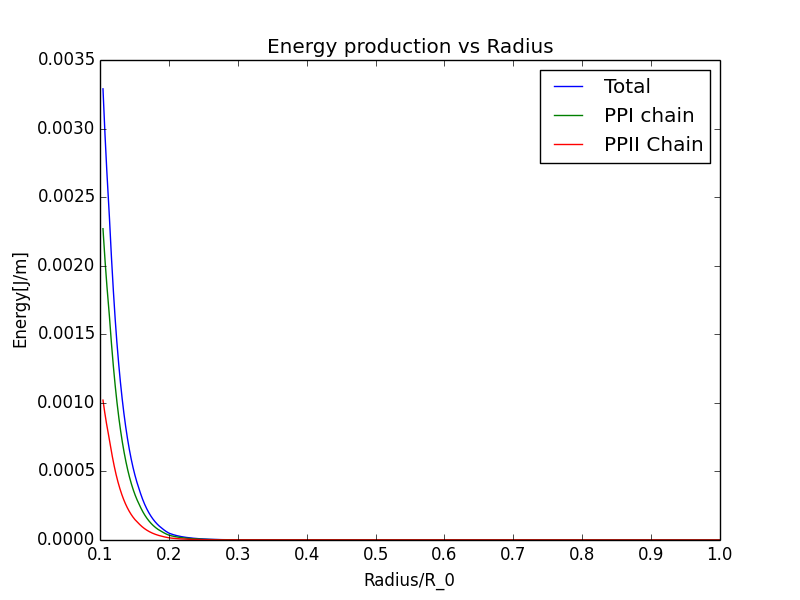
\includegraphics[width=\textwidth]{energyproduction}
\caption{Plot confirming expectations for energy production.}
\label{fig:Energy pruduction}
\end{figure}
To further check that this is the case we can plot the fractions of each divided by the total production. This produces the plot in figure \ref{fig:energyproduction_frac}, confirming what we expected. 
\begin{figure}[H]
	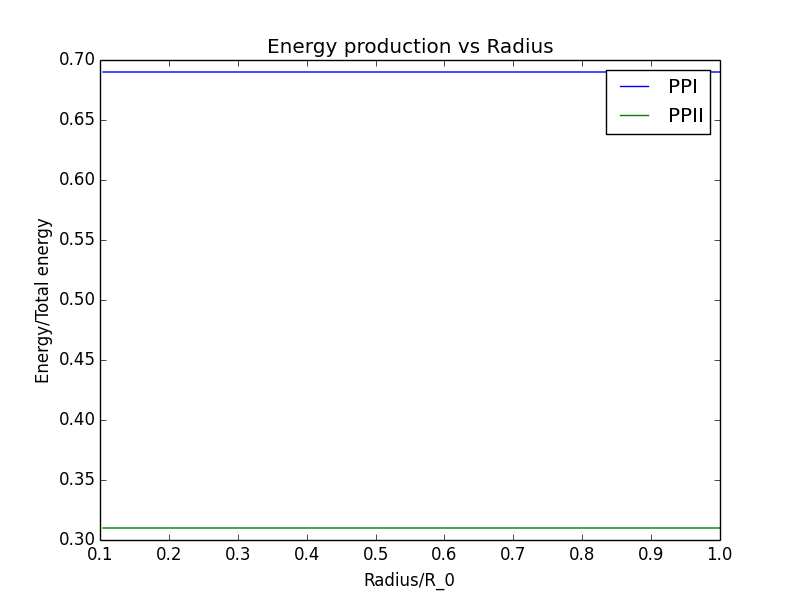
\includegraphics[width=\textwidth]{energyproduction_frac}
	\caption{Plot of the fractions produced by each of the PP chains.}
	\label{fig:energyproduction_frac}
\end{figure}

Since the first part of each of the chains dominates, it would be interesting to see how much the rest of the processes contribute to the fractions. This can be seen in figure \ref{fig:energyproduction_frac_only}. It is important to note that this plot doesn't really tell us anything productive before we reach a radius near the core, since the energy production is negligible at larger radii than that. It is still interesting to see that the second part of the PPII chain is more effective than the second part of the PPI chain near the core. If the PPII chain happened as much as the PPI chain, we would see a tiny difference between the two.
\begin{figure}[H]
	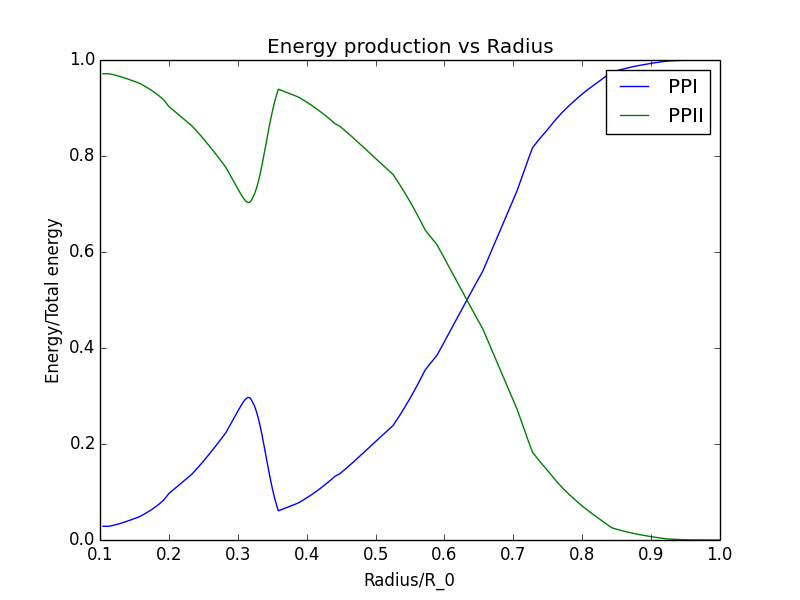
\includegraphics[width=\textwidth]{energyproduction_frac_only}
	\caption{Plot of the fractions produced by each of the PP chains without the prerequisites.}
	\label{fig:energyproduction_frac_only}
\end{figure}
\subsection{Energy transport}
In the sun we have the radiative zone on top of the core, and the convective zone on top of that. This means that the energy should be transported by convection at the surface, and as we approach the center, there should be a switch to transport by radiation. According to the lecture notes, the bottom of the convection zone is at $R = 0.72R_{\odot}$, and thus I expect to see a smooth transition between the two around this point.
This is not what we see in the model. Instead we see convection dominating from the start, and then being reduced to the same as radiation at about $R = 0.975R_{\odot}$, and then going to zero at $R = 0.95R_{\odot}$. We also see a number of jumps as we go further into the star. One could argue that one should expect some points inward where the gas is convectively unstable, and that would produce these spikes, but I wouldn't expect these rough transitions . All of this can be seen in figure \ref{fig:Energy transport}.
\begin{figure}[H]
	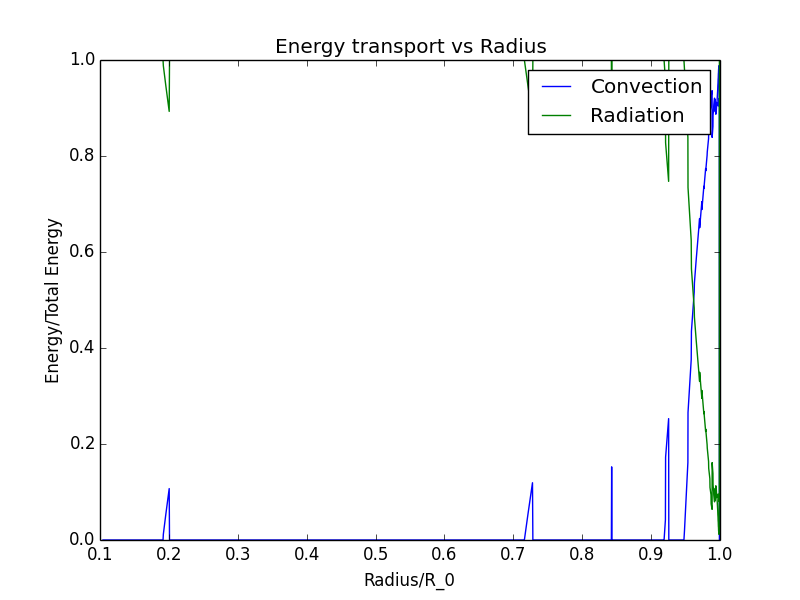
\includegraphics[width=\textwidth]{energytransport}
	\caption{Plot of energy transport.}
	\label{fig:Energy transport}
\end{figure}
\subsection{Mass}
The graph for the mass should be fairly flat in the beginning, and make an exponential fall as we approach the center. This becomes clear if we consider what happens as we move from the edge of the star towards the center. At the surface, the pressure is very small, and so the matter doesn't get forced together as much, resulting in a fairly low density. As we approach the center the pressure should grow enormously, resulting in an increase in density, which means that most of the matter in the sun is located close to the center.
The graph seen in figure \ref{fig:Mass} confirms this.
\begin{figure}[H]
	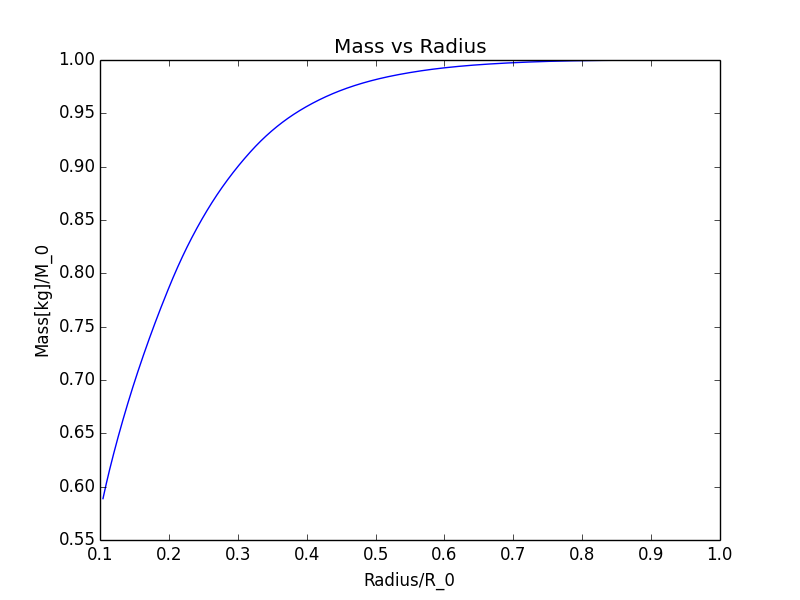
\includegraphics[width=\textwidth]{mass}
	\caption{Graph confirming expectations for the distribution of mass.}
	\label{fig:Mass}
\end{figure}
I actually don't know if this is realistic or not. The only place I could find any information about how much mass is in the core of the sun was Wikipedia, but they don't provide any references of where they get their values so I don't want to use them.
As I wrote above, we do expect a fairly large portion of the matter to be in the core, but I'm not sure we would expect 60\% of the mass inside 10\% of the radius. That does seem a bit too large.
\subsection{Pressure}
As was described in the section for mass, the pressure should be low at the surface of the sun, and as we decrease the radius, and approach the core, it should grow exponentially. This is confirmed by the graph in figure \ref{fig:Pressure}
\begin{figure}[H]
	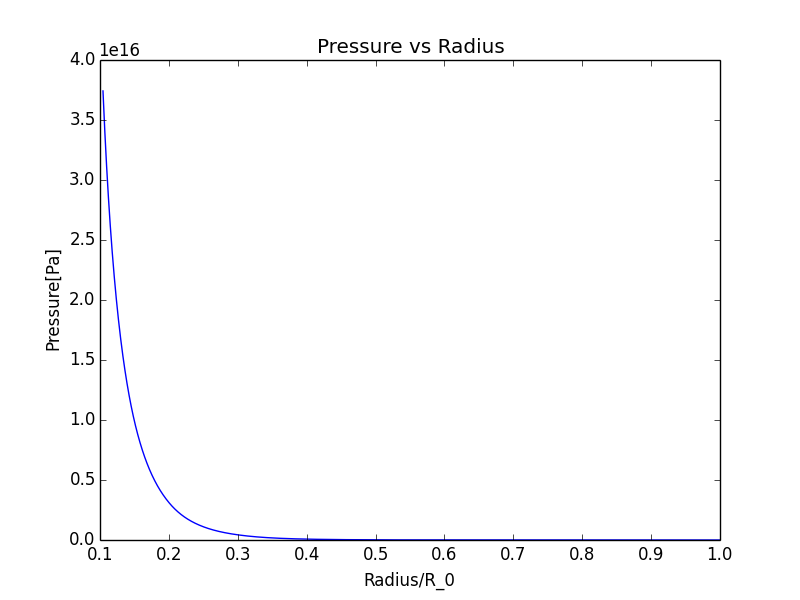
\includegraphics[width=\textwidth]{pressure}
	\caption{Graph confirming expectations for pressure.}
	\label{fig:Pressure}
\end{figure}
We see that the pressure ends up at about $3.75\times10^{16} Pa$ which is fairly close to the value given for the core in the lecture notes of $3.45\times10^{16} Pa$.
\subsection{Density}
The density should, like I described earlier, be low at the surface of the sun, and as we decrease the radius it should grow to values far exceeding those at the surface. When we look at figure \ref{fig:Density}, this is exactly what we see. 
\begin{figure}[H]
	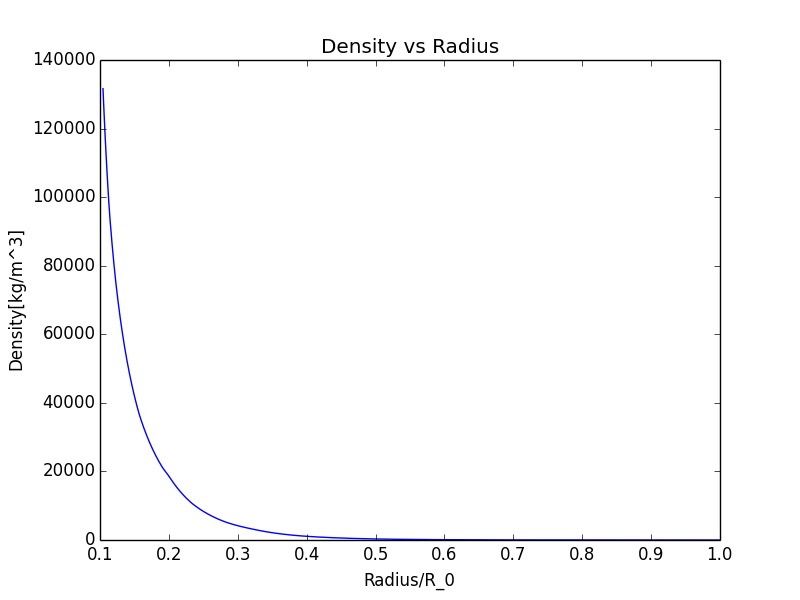
\includegraphics[width=\textwidth]{density}
	\caption{Graph confirming expectations for density.}
	\label{fig:Density}
\end{figure}
In fact we end up with a density of about $1.3\times10^5 kg/m^3$ which is very close to the value $1.62\times10^5 kg/m^3$ given for the core in the lecture notes.
\subsection{Temperature}
Since the only difference between this project and the first one is that we've added the convection zone, the temperature graph should look like it did in project 1 for the radiative zone. It should be noted that some mistakes were made in project 1, which could have affected the graph for temperature, and thus I can not be sure if any differences are due to mistakes in this model, or if they are from mistakes in the first project. 
The resulting plot from the program can be seen in figure \ref{fig:Temperature}.
\begin{figure}[H]
	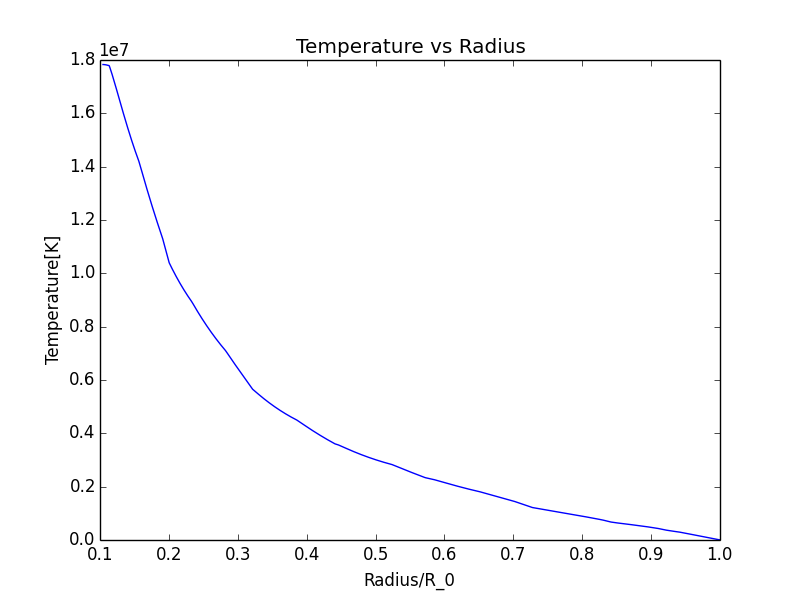
\includegraphics[width=\textwidth]{temperature}
	\caption{Plot of the temperature.}
	\label{fig:Temperature}
\end{figure}
Even though the graph for the temperature isn't very smooth we actually get a sensible result when approaching the core. From the plot we see that we stop at a value of about $1.8\times10^7 K$, and the actual value given for the core in the lecture notes is $1.57\times10^7 K$. However I did not expect such a rough graph for the temperature. That doesn't necessarily mean that it is wrong. It just means that there are some points where the temperature changes rapidly, which is to be expected if the transportation method changes. I don't recognize the graph for the radiative zone either. This leads me to think that there may be something wrong here, but since I get results that are consistent with the values one expects for the sun, I'll have to accept that the temperature should actually behave this way. 

\section{Conclusion}
In this model we've seen that when using the assumptions described in project 1 and in the section in this project, we can actually make a model that gives results that are consistent with the measured values for the sun. 

Most of the plots generated described reasonable behavior for the different physical quantities. There were however some variation from the expected behavior for the energy transport in the sun, and for the temperature. And we didn't get values that matched the ones from the lecture notes perfectly.

Even so, the model is fairly close to producing values equal to those observed in reality, and thus it is a good model even though there are some limitations to it.

\section{Collaboration}
During the first project, I asked Maria about a lot of things, and so the similarities between those projects are probably still in this project.
I have asked both Vigdis and Maria about many things during the course of this project, so I expect there to be some similarities in our approaches, but I haven't seen their programs so there shouldn't be anything similar there (except for the parts that were made for project 1). Peder also asked for some tips on how to make the energy function work as intended, and so I've shown him how this part of my program works. 

\section{Appendix}
\subsection{The python code}
\begin{verbatim}
"""
Term Project 2
The second term project now involves using Chap.5 to include convection
in your model of a star. In the first term project you modeled the sun from
its core to the edge if its radiative zone. Now you can include the rest of the
sun by including energy transport through convection. You should use the
model you have already done, but now include a check at each radius (or
mass) shell of convective stability. In case the shell is not convectively stable,
you need to use the equation for convective transport instead of radiative
transport. That involves solving Exerc. 5.10, to get the expression for the
convective flux, and through that get the temperature gradient. You can
make the same assumptions as in the first term project, for instance only
include PPI and PPII etc.

The project can be found at 
http://www.uio.no/studier/emner/matnat/astro/AST3310/v15/notes/exerc2.pdf

Created by Andreas Ellewsen
"""
from numpy import exp,zeros\
,genfromtxt,log10,pi,array,roots,imag,real    #Numerical python

from matplotlib.pyplot import plot,figure\
,title,xlabel,ylabel,show,hold,legend,savefig	#Plotting library

import sys as sys	#System functions

#Constants
G	= 6.67384E-11		#[m**3*kg**-1*s**-2] Gravitational constant
m_u 	= 1.66053892173E-27 	#[kg] Atomic mass unit
N_A 	= 6.0221413E23      	#[] Avogadros number
k   	= 1.3806488E-23		#[m**2*kg*s**-2*K**-1] Boltzmans constant
c	= 2.99792458E8		#[m*s**-1] Speed of lights in vacuum
sigma   = 5.67E-8		#[W*m**-2*K**-4] Stefan-Boltzmans constant
MeVtoJ 	= 1.60217657E-13 	#[J] Conversion factor from MeV to Joules
L_sun  	= 3.846E26		#[W] Luminosity of the sun
R_sun  	= 6.958E8		#[m] Radius of the sun
M_sun  	= 1.989E30		#[kg] Mass of the sun
alpha  = 1
#Energy output of reactions
Q_pp = (.15+1.02)  *MeVtoJ	#[J]
Q_dp = (5.49)	   *MeVtoJ	#[J]
Q_33 = (12.86)	   *MeVtoJ	#[J]
Q_34 = (1.59)	   *MeVtoJ	#[J]
Q_7e = (.05)	   *MeVtoJ	#[J]
Q_71prime = (17.35)*MeVtoJ	#[J]

#Initial conditions
X       = .7      #[] Hydrogen fraction
Y3      = 1E-10   #[] Helium 3 fraction
Y       = .29     #[] Sum of Helium 3 and Helium 4 fractions
Y4      = Y-Y3    #[] Helium 4 fraction
Z_73Li  = 1E-13   #[] Lithium  fraction
Z_74Be  = 1E-13   #[] Berylium fraction
Z       = .01		#[] Other
L_0     = L_sun   #[W] Luminosity of the star
R_0     = R_sun   	#[m] Radius of the star
M_0     = M_sun	#[kg] Mass of star 
rho_0   = 4E-4		#[kg*m**-3] Mass density of star 
P_0     = 1E8     #[Pa] Test value for pressure
T_0     = 5770	  	#[K] Temperature
nabla_ad = 2./5   #Adiabatic gradient for fully ionized ideal gas

#Computes number of atoms of the different elements.
def atomnumbers(rho):
n_e   = rho*(1+X) /(2.*m_u)    	#Number of electrons
n_d   = 0			#Number of deuterium atoms
n_p   = rho*X	  /m_u     	#Number of Hydrogen atoms
n_3   = rho*Y3	  /(3.*m_u)     #Number of Helium 3 atoms
n_4   = rho*Y4	  /(4.*m_u)     #Number of Helium 4 atoms
n_Li  = rho*Z_73Li/(7.*m_u) 	#Numver of Beryllium 7 atoms
n_Be  = rho*Z_74Be/(7.*m_u) 	#Number of Lithium 7 atoms
atomnumbers = [n_e,n_d,n_p,n_3,n_4,n_Li,n_Be]
return atomnumbers

#Reactions
"""In this part the reaction rates of the processes in the PPI and PPII \
chain are calculated. I neglect the other processes since I choose to \
look at a star with low temperature at it's core, and in that case those \
processes are very slow compared to PPI and PPII."""

def reactions(T):
T9 		= T*1E-9		#Convert T to form used in reactions.
T9_star1 	= T9/(1+4.95E-2*T9)	#Other form used.
T9_star2 	= T9/(1+.759*T9)	#Yet another form used.

H_D   	= 	4.01E-15*T9**(-2./3)*exp(-3.380*T9**(-1./3))*(1 +\
.123*T9**(1./3) + 1.09*T9**(2./3) + .938*T9)

He3_p	= 	6.04E10*T9**(-2./3)*exp(-12.276*T9**(-1./3))*(1 +\
.034*T9**(1./3) - .522*T9**(2./3)-.124*T9 + \
.353*T9**(4./3)+ .213*T9**(-5./3))

He3_Be  = 	5.61E6*T9_star1**(5./6)*T9**(-3./2)*exp(-12.826*\
T9_star1**(-1./3))

Be_Li   = 	1.34E-10*T9**(-1./2)*(1 - .537*T9**(1./3)  + \
3.86*T9**(2./3) +  .0027*T9**-1*exp(2.515E-3*T9**-1))

Li_p	= 	1.096E9*T9**(-2./3)*exp(-8.472*T9**(-1./3)) - \
4.830E8*T9_star2**(5./6)*T9**(-3./2)*exp(-8.472*\
T9_star2**(-1./3)) + 1.06E10*T9**(-3./2)\
*exp(-30.442*T9**-1)
"""
"These two reactions are not used in this assignment, but may be useful \
at a later point, so I've kept them here."

Berylliym_Boron = 	3.11E5*T9**(-2./3)*exp(-10.262*T9**(-1./3))+2.53E3\
*T9**(-3./2)*exp(-7.306*T9**-1)

Nitrogen_Oxygen = 	4.9E7*T9**(-2./3)*exp(-15.228*T9**(-1./3)-\
.092*T9**2)*(1+.027*T9**(1./3)-.778*T9**(2./3)\
-.149*T9+.261*T9**(4./3)+.127*T9**(5./3)) + \
2.37E3*T9**(2./3)*exp(-3.011*T9**-1) + \
2.19E4*exp(-12.53*T9**-1)
"""
rrs = [H_D,He3_p,He3_Be,Be_Li,Li_p]#,Berylliym_Boron,Nitrogen_Oxygen
return rrs

#Computing reactionrates
"""
This segment computes the reactionrates for the different processes in the sun.
"""
def Reactionrates(T,rho):
n = atomnumbers(rho)
rrs = reactions(T)

#Reaction rates
"""All of the following rates are calculated by the equation
r_ik = n_i*n_k/(rho*(1+delta_ik)*lambda_ik)
where i,k define the elements and delta_ik =1 if i=k else 0.
"""
lambda_pp = rrs[0]/N_A*1E-6		#[m^3/s]
lambda_33 = rrs[1]/N_A*1E-6		#[m^3/s]
lambda_34 = rrs[2]/N_A*1E-6		#[m^3/s]
lambda_7e = rrs[3]/N_A*1E-6		#[m^3/s]
lambda_71prime  = rrs[4]/N_A*1E-6	#[m^3/s]

r_pp 	  = n[2]**2/(rho*2)*lambda_pp	#[kg-1*s-1]
r_pd  	  = r_pp			#[kg-1*s-1] Assume this reaction happens \
#instantly such that it happens at the same \
#rate as the elements it needs become available.
#Thus it must be the same as the reaction that \
#creates those elements (in this case Deuterium)
r_33 	  = n[3]**2  /(rho*2)*lambda_33	#[kg-1*s-1]
r_34 	  = n[3]*n[4]/rho*lambda_34	#[kg-1*s-1]
r_7e 	  = n[5]*n[6]/rho*lambda_7e	#[kg-1*s-1]
r_71prime = n[5]*n[2]/rho*lambda_71prime#[kg-1*s-1]

#This part makes sure that reaction rates which rely on other rates \
#don't use elements that are not yet present.
if 2.*r_33 + r_34 > r_pd:
r_33 = 2./3*r_pd
r_34 = 1./3*r_pd
if r_7e > r_34:
r_7e = r_34
if r_71prime > r_7e:
r_71prime = r_7e
reactionrate = r_pp,r_pd,r_33,r_34,r_7e,r_71prime
return reactionrate

#Solving the equation for the change in Luminosity

def Energy(T,rho):
reactionrate = Reactionrates(T,rho)
e_1  = reactionrate[0]*(Q_pp+Q_dp)
e_2  = reactionrate[2]*Q_33
e_3  = reactionrate[3]*Q_34
e_4  = reactionrate[4]*Q_7e
e_5  = reactionrate[5]*Q_71prime
e    = e_1 + e_2 + e_3 + e_4 + e_5
PPI_frac  = e_2 + .69*e_1
PPII_frac = e_3 + e_4 + e_5 + .31*e_1 
PPI_only = e_2
PPII_only = e_3 +e_4+e_5
output = e,PPI_frac,PPII_frac,PPI_only,PPII_only
return output

#Defining functions for pressure,temperature and density
"""This part solves the equation for Pressure, assuming 
the equation of state to be that of an ideal gas"""

#Constants needed
mu 	= 1/(2.*X + 7./4*Y + 5./7*Z_74Be + 4./7*Z_73Li + Z)
a 	= 4.*sigma/c

def Pressure(rho,T):
P_rad 	= a/.3*T**4           #Radiation pressure
P_G 	= rho*k*T/(mu*m_u)    #Gas pressure, assuming ideal gas
P	= P_G + P_rad            #Total Pressure
return P

def Density(P,T):
rho  = (P*mu*m_u)/(k*T)		#Ideal gas
return rho

#Function that reads the opacity table
lines = genfromtxt('opacity.txt')

def Opacity(T,rho):
'''This function reads the opacity table'''
#Convert R and T to the form used in opacity.txt
R      = (rho*1E-3)/(T/1E6) 
Rvalue = log10(R)
Tvalue = log10(T)
Rvalue = (round(2*Rvalue)/2.)
#Print errormessage if using values outside table
if Rvalue >= 1.5 or Rvalue <= -8.5:
print 'Tried using R outside opacity table'
sys.exit()
if Tvalue >= 8.8 or Tvalue <= 3.7 :
print 'Tried using T outside opacity table'
sys.exit()

#Pick the right R value from the table
for i in range(len(lines[0])):
if Rvalue == lines[0][i]:
Ri = i

#Make list of T values found in table
Tlist = zeros(len(lines))
for i in range(1,len(lines)):
Tlist[i] = lines[i][0]

#Pick the right T value from the table
Ti = min(range(len(Tlist)), key=lambda i: abs(Tlist[i]-Tvalue))

#Pick the right kappa value with R and T
log10kappa = lines[Ti][Ri]

#Convert the value given to the form used in the equations
kappa = .1*10.**(log10kappa)
return kappa

#Solving the equations dictating the physics of the sun.
'''This is the part of the program that actually solves the equations\
governing the sun.'''

#Make empty lists
R = []
L = []
P = []
T = []
M = []
rho = []
epsilon = []
F_C = []
F_R = []
Convection_frac = []
Radiation_frac = []
PPI_fraction = []
PPII_fraction = []
PPI_only = []
PPII_only =[]
PPI_frac = []
PPII_frac = []

#Fill the lists with the initial conditions
M.append(M_0)
R.append(R_0)
L.append(L_0)
T.append(T_0)
rho.append(rho_0)
P.append(Pressure(rho[0],T[0]))
epsilon.append(Energy(T[0],rho[0])[0])


#Function to calculate xi
def xifunc(l_m,U,nabla_ad,nabla_rad):
c1 = l_m**2 / U
c2 = 1
c3 = 4*U/l_m**2
c4 = nabla_ad -nabla_rad
xi = roots([c1,c2,c3,c4])
for element in xi:
if imag(element) == 0:
xi = real(element)
break
return xi

#Simulate evolution by reducing radius.
i = 0    #Starts a counter
p = 0.01 #Max change allowed per step.

while M[i] > 0 and R[i] > 0 and L[i] > 0 and T[i] > 0 and P[i] > 0:
#Change in radius
dMdr	= 4*pi*R[i]**2*rho[i]
drM 	= p*M[i]/dMdr   #Largest dr allowed

#change in Pressure
dPdr 	= -(G*M[i]*rho[i])/R[i]**2
drP 	= p*P[i]/dPdr    #Largest dr allowed

#Change in Luminosity
dLdr 	= epsilon[i]*dMdr
drL 	= p*L[i]/dLdr  #Largest dr allowed

#Calculate the gradients
g       = G*M[i]/R[i]**2    #Gravitational acceleration at radius R
kappa   = Opacity(T[i],rho[i])		#Opacity
c_P     = 5./2*P[i]/(rho[i]*T[i])	#Heat capacity constant pressure
H_P     = P[i]*R[i]**2 / (G*M[i]*rho[i])	#Pressure scale height
l_m     = alpha*H_P	                #Mixing length
U       = 64*sigma*T[i]**3/(3*kappa*rho[i]**2*c_P)*(H_P/g)**(1./2)
nabla_rad  = 3*kappa*L[i]*P[i]/(64*pi*sigma*G*T[i]**4*M[i])

#Calculate xi
xi = xifunc(l_m,U,nabla_ad,nabla_rad)
#Calculate variables depening on xi
#v = (g*l_m**2/(4*H_P))**(1./2)*xi
nabla      = nabla_rad - l_m**2 / U *xi**3
nabla_star = nabla - xi**2


"""#Print test values
print 'nabla_rad  = ',nabla_rad
print 'nabla_ad   = ',nabla_ad
print 'nabla      = ',nabla
print 'nabla_star = ',nabla_star"""

#Change in temperature    
'Instability criterion deciding which gradient to use.'
if nabla_rad > nabla_ad:
dTdr = -T[i]/H_P*nabla
F_R.append(-16./3*sigma*T[i]**3/(kappa*rho[i])*dTdr)
F_C.append(L[i]/(4*pi*R[i]**2)-F_R[i])
else:
dTdr = -T[i]/H_P*nabla_rad
F_C.append(0)
F_R.append(-16./3*sigma*T[i]**3/(kappa*rho[i])*dTdr)
drT 	= p*T[i]/dTdr  #Largest dr allowed

#Decide how small dr needs to be
drR =   10*p*R[i]
dr  =   -min(abs(drR),abs(drP),abs(drL),abs(drT),abs(drM))
if abs(dr) < 1E2:
dr = -1E2   #Limit how small dr is allowed to become

#Update values
M.append(M[i] + dMdr*dr)		#Update Mass
R.append(R[i] + dr)     		#Update Radius
L.append(L[i] + dLdr*dr) 		#Update Luminosity
P.append(P[i] + dPdr*dr)		#Update Pressure
T.append(T[i] + dTdr*dr)		#Update Temperature
rho.append(Density(P[i],T[i]))	#Update Density
epsilon.append(Energy(T[i],rho[i])[0]) #Update Energy output
PPI_fraction.append(Energy(T[i],rho[i])[1]) #PPI of total
PPII_fraction.append(Energy(T[i],rho[i])[2]) #PPII of total
PPI_only.append(Energy(T[i],rho[i])[3]) #PPI without start
PPII_only.append(Energy(T[i],rho[i])[4]) #PPII without start
Convection_frac.append(F_C[i]/(F_C[i]+F_R[i])) #Convection fraction
Radiation_frac.append(F_R[i]/(F_C[i]+F_R[i])) #Radiation fraction

"""print 'M = %.3e, R = %.3e, L = %.3e, P = %.3e, T= %.3e, rho = %.3e, \
kappa = %.3e, epsilon = %.3e, dT = %.3e, dr = %.3e, dL = %.3e, dm = %.3e, \
dP = %.3e, F_C = %.3e, F_R = %.3e'%(M[i], R[i], L[i], P[i], T[i], rho[i], \
kappa, epsilon[i], dTdr*dr, dr, dLdr*dr, dMdr*dr, dPdr*dr,F_C,F_R)"""

#Print  information about which variable went to zero first.   
if M[i+1] < 0:
print 'Mass went negative'
if R[i+1] < 0:
print 'Radius went negative'
if L[i+1] < 0:
print 'Luminosity went negative'
if T[i+1] < 0:
print 'Temperature went negative'
if P[i+1] < 0:
print 'Pressure went negative'

i +=1   #increase counter

#Fractions of the total production for each of the chains.
PPI_fraction = array(PPI_fraction)
PPII_fraction = array(PPII_fraction)
PPI_frac = PPI_fraction/(PPI_fraction + PPII_fraction)
PPII_frac = PPII_fraction/(PPI_fraction + PPII_fraction)

#Fraction of the total prodcution for each of the chains without
#the prerequisites.
PPI_only = array(PPI_only)
PPII_only = array(PPII_only)
PPI_only_frac = PPI_only/(PPI_only + PPII_only)
PPII_only_frac = PPII_only/(PPI_only + PPII_only)

#Removes the lat set of results since they are unphysical
del M[-1]
del R[-1]
del L[-1]
del P[-1]
del T[-1]
del rho[-1]
del epsilon[-1]

#Print start values used in this run
print 'Start values:'
print 'M_0 :		   %.3e'%(M[0])
print 'R_0 :		   %.3e'%(R[0])
print 'L_0 :		   %.3e'%(L[0])
print 'P_0 :		   %.3e'%(P[0])
print 'T_0 :		   %.3e'%(T[0])
print 'rho_0 :		   %.3e'%(rho[0])
print 'epsilon_0:	   %.3e'%(epsilon[0])
print 'F_C: ', F_C[0]
print 'F_R: ', F_R[0]

#Scale values after initial conditions
M = array(M)/M[0]
R = array(R)/R[0]
L = array(L)/L[0]

#print Final values
print 'Final values:'
print 'M/M_0 :		   %.3f'%(M[-1])
print 'R/R_0 :		   %.3f'%(R[-1])
print 'L/L_0 :		   %.3f'%(L[-1])
print 'P : 		   %.3e'%(P[-1])
print 'T :  		   %.3e'%(T[-1])
print 'rho   :       %.3e'%(rho[-1])
print 'epsilon:	   %.3e'%(epsilon[-1])
print 'F_C: ', F_C[-1]
print 'F_R: ', F_R[-1]

#Plots of interesting things
figure()
plot(R,M)
title('Mass vs Radius')
xlabel('Radius/R_0')
ylabel('Mass[kg]/M_0')
savefig('mass.png')

figure()
plot(R,P)
title('Pressure vs Radius')
xlabel('Radius/R_0')
ylabel('Pressure[Pa]')
savefig('pressure.png')

figure()
plot(R,L)
title('Luminosity vs Radius')
xlabel('Radius/R_0')
ylabel('Luminosity/L_0')
savefig('luminosity.png')

figure()
plot(R,T)
title('Temperature vs Radius')
xlabel('Radius/R_0')
ylabel('Temperature[K]')
savefig('temperature.png')

figure()
plot(R,rho)
title('Density vs Radius')
xlabel('Radius/R_0')
ylabel('Density[kg/m^3]')
savefig('density.png')

figure()
plot(R,Convection_frac)
title('Energy transport vs Radius')
xlabel('Radius/R_0')
ylabel('Energy/Total Energy')
hold('on')
plot(R,Radiation_frac)
legend(['Convection','Radiation'])
hold('off')
savefig('energytransport.png')

figure()
plot(R,epsilon)
title('Energy production vs Radius')
xlabel('Radius/R_0')
ylabel('Energy[J/m]')
hold('on')
plot(R,PPI_fraction)
plot(R,PPII_fraction)
legend(['Total','PPI chain','PPII Chain'])
hold('off')
savefig('energyproduction.png')

figure()
plot(R,F_C)
title('Energy transport vs Radius')
xlabel('Radius/R_0')
ylabel('Energy[W/m^2]')
hold('on')
plot(R,F_R)
legend(['Convection','Radiation'])
hold('off')
savefig('energytransport_frac.png')

figure()
plot(R,PPI_frac)
title('Energy production vs Radius')
xlabel('Radius/R_0')
ylabel('Energy/Total energy')
hold('on')
plot(R,PPII_frac)
legend(['PPI','PPII'])
hold('off')
savefig('energyproduction_frac.png')


figure()
plot(R,PPI_only_frac)
title('Energy production vs Radius')
xlabel('Radius/R_0')
ylabel('Energy/Total energy')
hold('on')
plot(R,PPII_only_frac)
legend(['PPI','PPII'])
hold('off')
savefig('energyproduction_frac_only.png')

show()
\end{verbatim}
\end{document}